\yourname

\activitytitle{Union, intersection, Venn diagram, complement, difference}{}

\overview{An introduction to set unions and intersections, Venn diagrams to represent sets, and set complements and differences.
Co-authored by Johanson Berlie.}

% ======================================================================

\definition{Disjoint sets}{
If two sets $A$ and $B$ have no elements in common, we say that they are \textbf{disjoint} sets.
}

\example{
The set consisting of all World War II veterans and the set of all millennials are disjoint sets. 
}{0in}

\definition{Comparable sets}{
Two sets A and B are \textbf{comparable} if $A \subseteq B$ or $B \subseteq A$. If this is not the case, then they are said to be \textbf{not comparable}.
}

\example{
The sets A = \{General Motors, Toyota, Ford, Renault\} and B = \{Tesla, Fisker\} are not comparable.
If we define a set C = \{Ford, Toyota\}, then A and C are comparable, since $C \subseteq A$.
}{0in}

\exercise{
For the following questions, compare the sets in the context of the definitions above. 
Are they equal?
Are they disjoint?
Are they comparable?
Is one a subset of the other?
In every case, explain why.
\balist{0.2in}

\item The set $A$ of US citizens and the set $B$ of people in the US right now.
    
\item Think of the set $A$ of US citizens and the set $J$ of citizens of Japan.  Do they have any elements in common, or are they disjoint?
This might require an internet search.

\item The set $A = \{ \divideontimes, \boxtimes, \blacktriangleleft, \boxplus \} $ and the set $B = \{ \boxplus, \blacktriangleleft, \divideontimes, \boxtimes \} $
    
\item The set of humans that have been to more than one planet and the set of humans that have been to Pluto.
    
\item The set $G$ consisting of the members of the Green Bay Packers on the first play of a game and the set $M$ consisting of the members of the Manchester United soccer team in play during a game.
    
\item The set $J$ consisting of all employees of the Department of Justice and the set $F$ consisting of all federal employees.

\item Suppose you know that $A \subseteq B$ and also that $B \subseteq A$.
What more can you say about $A$ and $B$ now?
Why?
    
\item Is it possible for the universal set to be disjoint from any of its subsets? Explain why or why not.
   
\elist
}{0.1in}

%\definition{}{
%When the objects of a set are set themselves, we call them a \textbf{family of sets} or a \textbf{class of sets}
%}

%\definition{}{
%the \textbf{power set} of any set S is the set of all subsets of S, including the empty set and S itself. The power set of a set S is usually denoted by \textbf{P(S)},
%}


% ======================================================================

\definition{Union of sets}{
The \textbf{union} of sets A and B is a new set, consisting of all elements which belong to A or to B or to both. We denote this by $A \cup B$.
}

\definition{Intersection of sets}{
The \textbf{intersection} of sets A and B is a new set, consisting of all elements which belong to both A and B. We denote this by $A \cap B$.
}

\example{
Let $C$ be the set of Computer Science majors and $M$ be the set of Mathematics majors.
Then $C \cap M$ is the set of students double majoring in Computer Science and Mathematics (a powerful combination!) while $C \cup M$ is the set of students majoring in one, the other, or both majors.
}{0in}

\exercise{ Answer the following, expressing the answers as sets where possible.
\balist{0.2in}
\item If $P=\{red, blue, yellow\}$, $S=\{purple, green, orange\}$, $M=\{red, green, blue\},$ find:
\item $P \cup S$
\item $P \cap M$
\item $P \cup S \cup M$
\item $P \cap S \cap M$
\item What is $A \cap A$? What about $A \cup A$?
\item Is it always true that $A \cup B=B \cup A$? Explain. 
\item If $A\subseteq B$ then what is $A \cup B$?
\item Is $A \cap B$ a subset of $A$? Is $A \cap B$ a subset of $B$? Explain.
\item What is $\varnothing \cap A$? Does it depend on the set $A$? Explain why or why not.
\item What is $\varnothing \cup A$? Does it depend on the set $A$? Explain why or why not. 
\item If $A \cup B=\varnothing$, can we say anything about $A$ or $B$? Is there something special about them? Explain.
\item If $A$ and $B$ are disjoint, what can we say about $A \cap B$?
\item If $A\subseteq B$ and $B$ and $C$ are disjoint, then what about $A$ and $C$?
\item If $U$ denotes the universal set, is it true that $U \cap A=A \cap \varnothing$? Explain.

\elist
}{0.1in}

% =====================================================================

\definition{Universal set}{
If all of the sets under discussion are subsets of a fixed set, this set is called the \textbf{universal set} or \textbf{universe of discourse} and denoted by \textbf{U}.
Sometimes there is more than one possibility for $U$.
}

\example{
If we were studying the citizenship of people around the world, the universal set would consist of all the people on earth.
Citizens of the US would be one interesting set, citizens of Canada would be another.
Do these two sets have any elements in common?  If so, how could that happen?
}{0in}

\example{
If we were studying binary stars, the universal set would be all the stars in the universe.
}{0in}

\exercise{~

\balist{0.2in}

\item When thinking of prime numbers, what is a good choice for the universal set?

\item When solving linear equations like $5x + 7 = 3$, what a good choice for the universal set?

\item When solving quadratic equations like $x^2 + 5x + 8 = 0$, what is the universal set?
    
\item Is it possible for the universal set to be empty? Explain why or why not.
    
\item If two sets $A$ and $B$ are subsets of a given universal set, $U$, is it possible that $A = U$ or $B = U$? Explain why or why not.
    
\elist
}{0.1in}


% ===================================================================
\definition{Venn diagram}{
A Venn diagram (also called \textbf{primary diagram}, \textbf{set diagram} or \textbf{logic diagram}) is a picture that shows all possible logical relations between a finite collection of sets. These diagrams depict elements as points in the plane, and sets as regions inside closed curves.
}

\remark{
This definition might seem complicated, but for our purposes we will think of Venn diagrams as circles that represent sets. The following examples will help make this clear.
}

\example{
To represent a single set using a Venn diagram, we draw a single circle (representing the set) inside a rectangle (representing the universal set).
We usually write the label for a given set inside the curve that represents it.
Note that the set $A$ could be empty but we still draw it with a circle; it may take a while to get used to that.

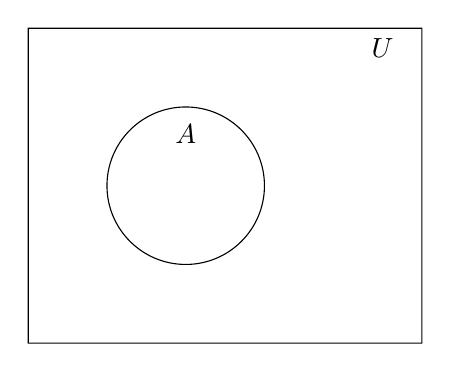
\begin{tikzpicture}[fill=gray]

% outline
\draw (0,0) circle (1) (0,0.9)  node [text=black,below] {$A$}
      (-2,-2) rectangle (3,2)  (2.5,1.5) node [text=black,above] {$U$};
\end{tikzpicture}
}{0in}

\example{
The representation in the above example can be extended to any finite number of sets. If want to represent two disjoint sets, A and B, we can represent them as below.

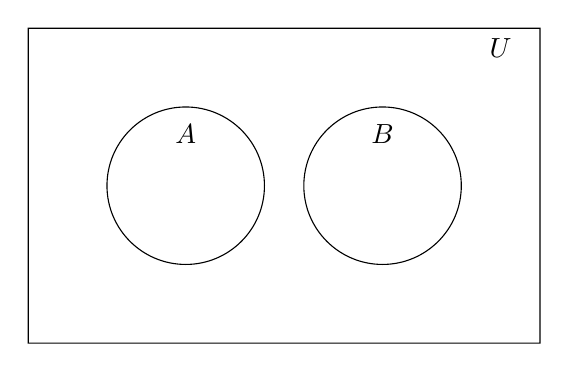
\begin{tikzpicture}[fill=gray]

% outline
\draw (0,0) circle (1) (0,0.9)  node [text=black,below] {$A$}
      (2.5,0) circle (1) (2.5,0.9)  node [text=black,below] {$B$}
      %(5,0) circle (1) (5,1)  node [text=black,above] {$C$}
      (-2,-2) rectangle (4.5,2)
      (4,1.5) node [text=black,above] {$U$};

\end{tikzpicture}

\noindent
The circles do not overlap, to indicate that the sets are disjoint.
Note that $A$ or $B$ or both could actually be empty sets, a bit like looking down into empty paper bags.

}{0in}


\remark{
The power of Venn diagrams is that they make it easy to understand set relations and operations. 
Let's look at a few examples.
}

\example{
If B is a subset of A, that is, if $B \subseteq A$ we can represent this as below.

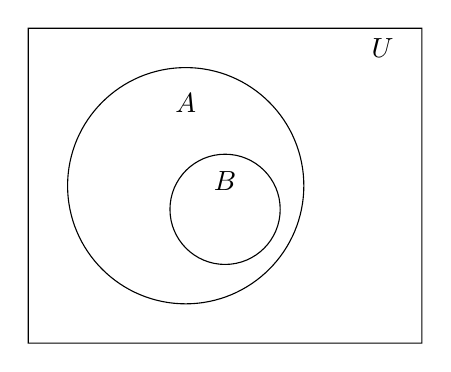
\begin{tikzpicture}[fill=gray]

% outline
\draw (0,0) circle (1.5) (0,1.3)  node [text=black,below] {$A$}
      (0.5,-0.3) circle (0.7) (0.5,0.3)  node [text=black,below] {$B$}
      (-2,-2) rectangle (3,2) (2.5,1.5) node [text=black,above] {$U$};
\end{tikzpicture}

\noindent
Note that it is possible that $B = A$; the blank areas in the diagram may or may not contain points; they may be empty.

}{0in}

\example{
If B is a proper subset of A, we can represent this with a dot outside B, but within A.

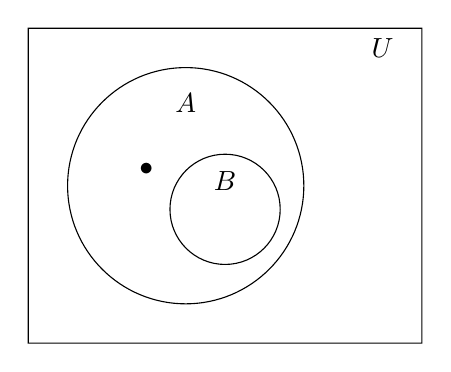
\begin{tikzpicture}[fill=gray]

% outline
\draw (0,0) circle (1.5) (0,1.3)  node [text=black,below] {$A$}
      (0.5,-0.3) circle (0.7) (0.5,0.3)  node [text=black,below] {$B$}
      (-0.5,0) node [text=black,above] {$\bullet$}
      (-2,-2) rectangle (3,2) (2.5,1.5) node [text=black,above] {$U$};
\end{tikzpicture}

\noindent
Now it's clear that every element of $B$ is also an element of $A$, but that there is an element of $A$ that is not an element of $B$.
It could be that $B$ is empty.
}{0in}


\example{
The generic picture of two sets $A$ and $B$ shows them overlapping, but not completely:

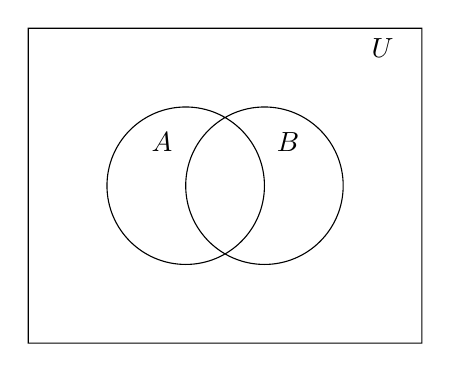
\begin{tikzpicture}[fill=gray]

% outline
\draw (0,0) circle (1) (-0.3,0.8)  node [text=black,below] {$A$}
      (1,0) circle (1) (1.3,0.8)  node [text=black,below] {$B$}
      (-2,-2) rectangle (3,2)  (2.5,1.5) node [text=black,above] {$U$};
\end{tikzpicture}

}{0in}


\example{
To indicate the intersection of $A$ and $B$, we shade $A \cap B$ as below, even if it is possible that the intersection is an empty set:

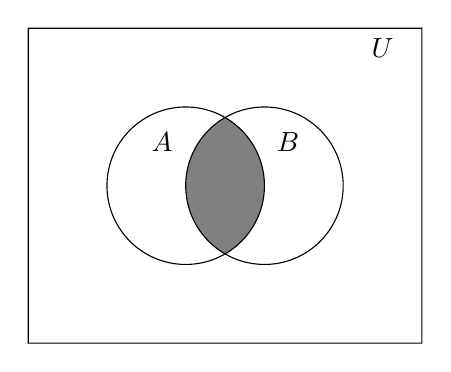
\begin{tikzpicture}[fill=gray]

\scope % A \cap B
\clip (0,0) circle (1);
\fill (1,0) circle (1);
\endscope

% outline
\draw (0,0) circle (1) (-0.3,0.8)  node [text=black,below] {$A$}
      (1,0) circle (1) (1.3,0.8)  node [text=black,below] {$B$}
      (-2,-2) rectangle (3,2)  (2.5,1.5) node [text=black,above] {$U$};
\end{tikzpicture}

}{0in}

\example{
If we know that A and B, are not disjoint, we indicate this by a dot inside the region of their overlap.


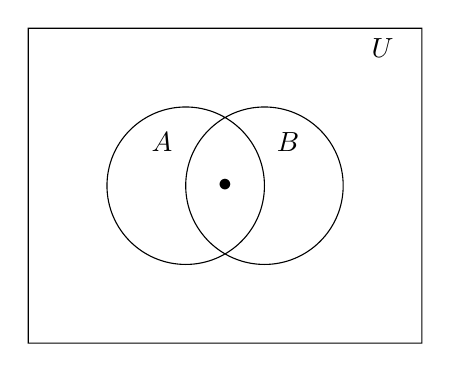
\begin{tikzpicture}[fill=gray]

\scope % A \cap B
\clip (0,0) circle (1);
%\fill (1,0) circle (1);
\endscope

% outline
\draw (0,0) circle (1) (-0.3,0.8)  node [text=black,below] {$A$}
      (1,0) circle (1) (1.3,0.8)  node [text=black,below] {$B$}
      (0.5,-0.2) node [text=black,above] {$\bullet$}
      (-2,-2) rectangle (3,2)  (2.5,1.5) node [text=black,above] {$U$};
\end{tikzpicture}

}{0in}


\example{
For two sets A and B, we represent $A \cup B$ as below:

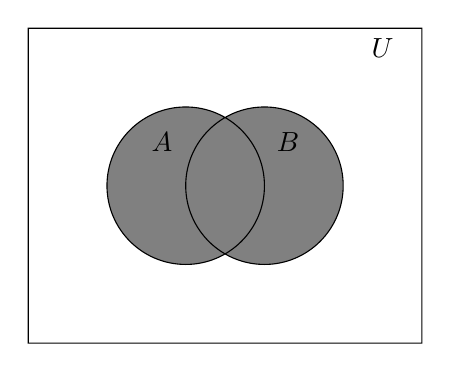
\begin{tikzpicture}[fill=gray]

\scope % A \cap B
\fill (1,0) circle (1);
\fill (0,0) circle (1);
\endscope

% outline
\draw (0,0) circle (1) (-0.3,0.8)  node [text=black,below] {$A$}
      (1,0) circle (1) (1.3,0.8)  node [text=black,below] {$B$}
      (-2,-2) rectangle (3,2)  (2.5,1.5) node [text=black,above] {$U$};
\end{tikzpicture}

}{0in}


\example{
For three sets A, B and C, we draw them to allow for all possible intersections.
We represent $A \cap B \cap C$ as below, even though it may actually be an empty set:

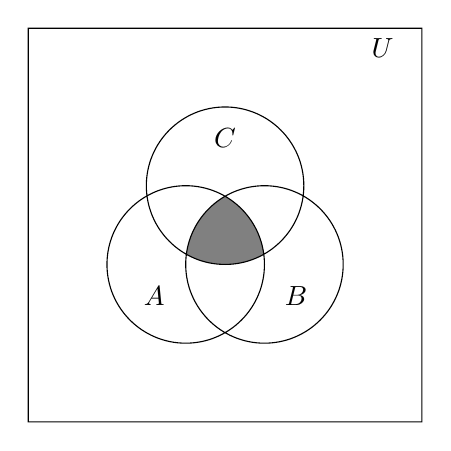
\begin{tikzpicture}[fill=gray]

\scope % A \cap B
\clip (0,0) circle (1);
\clip (0.5,1) circle (1);
\fill (1,0) circle (1);
\endscope

% outline
\draw (0,0) circle (1) (-0.4,-0.4)  node [text=black] {$A$}
      (1,0) circle (1) (1.4,-0.4)  node [text=black] {$B$}
      (0.5,1) circle (1) (0.5,1.6)  node [text=black] {$C$}
      (-2,-2) rectangle (3,3) (2.5,2.5) node [text=black,above] {$U$};
\end{tikzpicture}
}{0in}


\exercise{
For the following questions, represent your answers as Venn diagrams, where possible. If a Venn diagram is not possible, explain why.
\balist{0.8in}
    
\item Make a Venn diagram for sets $A$ and $B$, showing that $A$ and $B$ are disjoint, and shade $A \cup B$.
    
\item Make a Venn diagram for sets $A$, $B$, and $C$, showing that $B$ and $C$ are disjoint.
    Shade the set $(A\cap B)\cup C$.
    
\item Make a Venn diagram for sets $A$, $B$, and $C$, showing that $A \cap B \cap C$ is empty, and shading $(A \cap B) \cup (A \cap C) \cup (B \cap C)$.
    
\item Make a Venn diagram for sets $A$, $B$, and $C$, showing that $A$ and $B$ are not disjoint and that $C \subset B$ but $C$ is disjoint from $A$.  
    
\item Make a Venn diagram for sets $A$, $B$, and $C$, showing that $A \cap B \subset C$, but $C \subset A \cup B$.
    \vspace{8em}
    
    
\elist
}{0.4in}


% =====================================================================
\definition{Set complement}{
The \textbf{complement} of a set A is the set of elements that do not belong to A. 
Therefore, it is every element of the universal set $U$ that is not an element of $A$.
We denote the complement of A as $A^c$ or $A'$. 
Visually, we represent this as:

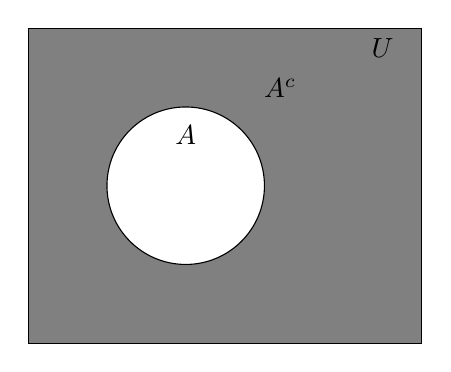
\begin{tikzpicture}[fill=gray]
\scope % A^c
    \filldraw   (-2,-2) rectangle (3,2) (2.5,1.5) node [text=black,above] {$U$};
    \fill[white] (0,0) circle (1);
\endscope
% outline
\draw (0,0) circle (1) (0,0.4)  node [text=black,above] {$A$}
      (1.2,1)  node [text=black,above] {$A^c$};
\end{tikzpicture}

}


\definition{Set difference}{  
The \textbf{difference} of sets A and B is the set of elements which belong to A but not to B. We denote this as $A-B$ or $A \setminus B$. Visually, we represent this by drawing $A$ and $B$ and shading the elements in $A$ but not in $B$.

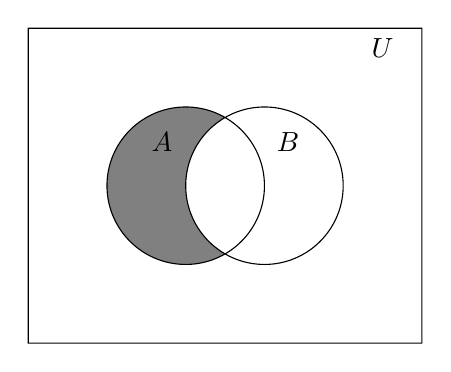
\begin{tikzpicture}[fill=gray]
% left hand
\scope
\clip (-2,-2) rectangle (2,2)
      (1,0) circle (1);
\fill (0,0) circle (1);
\endscope
% right hand
%\scope
%\clip (-2,-2) rectangle (2,2)
      %(0,0) circle (1);
%\fill (1,0) circle (1);
%\endscope
% outline
\draw (0,0) circle (1) (-0.3,0.8)  node [text=black,below] {$A$}
      (1,0) circle (1) (1.3,0.8)  node [text=black,below] {$B$}
      (-2,-2) rectangle (3,2) (2.5,1.5) node [text=black,above] {$U$};
\end{tikzpicture}

%TODO: explain difference of sets as relative complement

}

%TODO: add a remark explaining the concept of relative complement

%\definition{}{
%The \textbf{Cartesian product} of two sets A and B, denoted by A $\times$ B is the set of all ordered pairs $(a,b)$ where a $\in$ A and b $\in$ B. It can be specified using set-builder notation, i.e. $A \times B=\{(a,b) : a\in A$ and  $b\in B\}$.
%}


\exercise{
For the following questions, start by drawing a Venn diagram for sets $A$ and $B$, then shade the desired set or sets.
For more than one set, use different shading for each one.
\balist{0.8in}
    
\item $(A \cap B)^c$, given that $A$ and $B$ are not disjoint.
    
\item $(A^c \cup B^c)$, given that $A$ and $B$ are not disjoint.
    
\item $A^c$ and $A^c \setminus B$.
    
\item Supposing that $B \subset A$, shade in $A \setminus B$. 
       
\elist
}{0.0in}

